\chapter[Resultados Parciais]{Resultados Parciais}
Com o final da primeira etapa do trabalho (TCC1), deve-se fornecer algumas informações sobre o \textit{status} atual do projeto. Esse capítulo proporciona esse \textit{feedback}. O capítulo está organizado em seções. Na seção 6.1 são recapitulados os objetivos estipulados para a primeira etapa do projeto. Na seção 6.2 são apresentadas informações sobre as ações futuras, para a segunda etapa do projeto, no TCC2.

\section{\textit{Status} Atual}
As atividades previstas para a primeira fase do Trabalho de Conclusão de Curso foram executadas com sucesso. Verifica-se que o projeto está com 52,4\%  das suas atividades concluídas. Para essa análise, considerou-se as atividades descritas nos cronogramas, tendo as atividades previstas para a segunda parte do projeto um peso maior, com fator 2.
\par
\begin{figure}[h]
\centering
  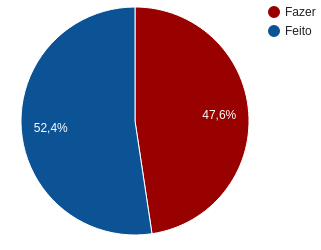
\includegraphics[width=0.5\textwidth]{figuras/pizzadobro.png}
  \caption{ \textit{Status} do Projeto}
  \label{fig:resultados}
\end{figure}
\par
\indent A Figura \ref{fig:resultados} apresenta um gráfico representando o \textit{status} do projeto, em termos de atividades, finalizados ou a fazer. Averiguando os cronogramas e o gráfico, observa-se que as atividades de levantamento de referencial, definição de escopo, configuração de ambiente e aquisição de conhecimento foram concluídas.
\par
\indent A revisão sobre verificação e validação de software, bem como sobre teste de software foi de grande valia, pois permitiu relembrar alguns aspectos e conceitos relacionados ao produto final do projeto: testes unitários. O aprendizado sobre \textit{frameworks} permitiu melhor entendimento sobre o assunto. A partir do conhecimento adquirido pode-se ter uma maior perspectiva a respeito de caracterização de \textit{frameworks}. Observar algumas técnicas de geração de teste permitiu identificar a forma candidata mais agradável para a produção de testes.
\par
\indent O trabalho também permitiu o estudo e utilização de ferramentas de automatização de configuração de ambiente. O uso do Vagrant para subir uma VM (\textit{Virtual Machine}) e de \textit{scripts} para configurá-lo, apenas com alguns comandos, tornou-se um prática importante no contexto do trabalho. Além disso, um aprendizado importante para a vida profissional.
\par
\indent Observa-se também que os objetivos almejados com a prova de conceito foram alcançados: geração de um teste para um método simples de adição de dois números, bem como a aquisição de conhecimento sobre Flexc++ e Bisonc++ e o uso prático delas. Além de permitir a prática da geração de testes, o que propiciou maior confiança no projeto.
\par
\indent A respeito de implementação já possui parte do analisador léxico e sintático, tanto da linguagem alvo, \textit{Grails}, quanto da notação candidata. Uma visão inicial da arquitetura do software também já é visível.

\section{Ações Futuras}
Para a próxima etapa do trabalho pretende-se completar o analisador léxico e sintático para a linguagem alvo, \textit{Grails}. É intenção também a evolução do gerador, permitindo a criação de testes para as tarefas básicas em aplicações \textit{web}, o CRUD. E, enfim, implementar a camada de customização do \textit{framework}, garantindo interfaces e pontos de extensão.